\section{Method}\label{sec:method}

\subsection{Derivation of the key equations}

To a very good approximation, stars in galaxies move as a collisionless fluid
that obeys the collisionless Boltzmann equation
\citep[e.g.][]{BinneyTremaine2008}:

\begin{equation}
\frac{\text{d}f}{\text{d}t} = \frac{\partial f}{\partial t} + \nabla_{\vec{x}} f\cdot\vec{v} - \nabla_{\vec{v}} f\cdot\nabla_{\vec{x}}\Phi = 0,
\end{equation}
where $f(\vec{x},\vec{v})$ is the distribution function of stars in phase space;
$\vec{x}$ and $\vec{v}$ are the position and velocity of the stars; and $\Phi$
is the gravitational potential.

In spherical coordinates $(r, \theta, \phi)$, the collisionless Boltzmann
equation becomes:

\begin{equation}
    \frac{\partial f}{\partial t} + \dot{r}\frac{\partial f}{\partial r} + \dot{\theta}\frac{\partial f}{\partial \theta} + \dot{\phi}\frac{\partial f}{\partial \phi} + \dot{v}_r\frac{\partial f}{\partial v_r}+\dot{v}_\theta\frac{\partial f}{\partial v_\theta} +\dot{v}_\phi\frac{\partial f}{\partial v_\phi} = 0
\label{eqn:colboltz}
\end{equation}
where $\dot{r} = v_r, \dot{\theta} = v_\theta$ and $\dot{\phi} = v_\phi / r
\sin\theta$ are the velocities in spherical coordinates.

In principle, given the positions and velocities of many stars we could directly
solve equation \ref{eqn:colboltz} for the force field $\nabla_{\vec{x}}\Phi$. In
practice, this is impractical as it involves derivatives of $f$ that is six
dimensional and thus very poorly sampled. One way around this problem is to use
instead velocity moments of equation \ref{eqn:colboltz} -- the Jeans equations
\citep[e.g.][]{BinneyTremaine2008}. Assuming a non-rotating steady state
($\partial f/\partial t=0$, $\langle {v}_r \rangle = \langle {v}_\theta \rangle
= \langle {v}_\phi \rangle =0$); spherical symmetry; and defining the tangential
velocity dispersion $\sigma_\phi^2 \equiv \sigma_\theta^2=\sigma_t^2$, the
second order moment is given by:

\begin{equation}\label{eqn:Jeans}
    \frac{1}{\nu}\frac{\partial}{\partial r}\left(\nu\sigma_{r}^2\right) +
    \frac{2\beta(r)\sigma_{r}^2}{r} = -\frac{\partial \Phi}{\partial r} &=& -\frac{GM(<r)}{r^2},\\
\end{equation}
where $M(<r)$ is the total cumulative mass; $\nu$ is the density of a set of
tracer star particles moving in the potential $\Phi(r)$; $G =
6.67398\cdot10^{-11} \text{m}^3/\text{kg}\,\text{s}^2$ is Newton's gravitational
constant; and $\beta$ is the
velocity anisotropy as in equation \ref{eqn:beta}.

Integrating both sides of equation \ref{eqn:Jeans} gives the radial velocity
dispersion as function of radius $r$, and correspondingly the fourth order
moment:

\begin{eqnarray}
    \sigma_r^2(r) & = & \frac{1}{\nu(r)}\exp\left(-2\int_{r_{\rm min}}^{r}
        \frac{\beta(s)}{s}\text{d}s\right)\cdot \nonumber \\
   & & \int_r^\infty \frac{GM(\tilde{r}r)\nu(\tilde{r})}{\tilde{r}^2}
   \exp\left(2\int_{r_{\rm min}}^{\tilde{r}}\frac{\beta(s)}{s}\text{d}s\right)
   \text{d}\tilde{r}
\label{eqn:main}
\end{eqnarray}
and:

\begin{eqnarray}
    \langle{v_r^4}\rangle(r) & = & \frac{3}{\nu(r)}\exp\left(-2\int_{r_{\rm min}}^{r}
        \frac{\beta'(s)}{s}\text{d}s\right)\cdot \nonumber \\
   & & \int_r^\infty \frac{GM(\tilde{r})\nu\sigma_r^2}{\tilde{r}^2}
   \exp\left(2\int_{r_{\rm min}}^{\tilde{r}}\frac{\beta'(s)}{s}\text{d}s\right)
   \text{d}\tilde{r}
\label{eqn:main4}
\end{eqnarray}
(Note that $r_{\rm min}$ leads to an integration constant that cancels and so
the choice of $r_{\rm min}$ is arbitrary.)

Typically, only {\it projected} velocities are observable. Projecting equations
\ref{eqn:main} and \ref{eqn:main4} along the line of sight, we obtain:

\begin{equation}
    \siglos^2(R) = \frac{2}{\Sigma(R)}\int_R^\infty \left(1-\beta\frac{R^2}{r^2}\right)
    \frac{\nu(r)\sigma_r^2(r) r}{\sqrt{r^2-R^2}}\text{d}r,
\label{eqn:LOS}
\end{equation}
where $\Sigma(R)$ denotes the surface mass density at {\it projected} radius
$R$.

From equation \ref{eqn:main}, it is clear that the velocity anisotropy
$\beta(r)$ trivially degenerates with the cumulative mass distribution $M(<r)$
that we would like to measure. This is problematic because with only line of
sight velocities $\beta(r)$ is poorly constrained, unless many thousands of
velocities are available \citep[e.g.][]{Wilkinson+2002}. This is one motivation
for considering the higher order moment equations: these may break the
$M(<r)-\beta(r)$ degeneracy. We will explore this later on in this paper, but
note that there is cause already for pessimism. For every higher order moment
equation, there are new `anisotropy parameters', in this case $\beta'$ -- the
hierarchy of Jeans equations are not closed
\citep[e.g.][]{BinneyTremaine2008}. Since each new equation adds yet another new
unknown, unless there are strong theoretical reasons for a relationship between
$\beta$, $\beta'$ and similar, the higher order moments are unlikely to yield
improved constraints \citep[e.g.][]{RichardsonFairbairn2013}. More promising are
the virial parameters discussed by \citep{RichardsonFairbairn2014} that involve
fourth order moments but are independent of $\beta'$. We will consider these in
a separate publication.

\subsection{The mass distribution}

In the following, we present a non-parametric method for the solution of
equation ~\ref{eqn:LOS} for the total gravitating mass
density $\rho(r)$, given a single or multiple tracer density profiles $\nu_i(r)$
with corresponding line-of-sight velocity dispersions $\siglosi(R)$. We write the overall density profile $\rho(r)$ as:

\begin{equation}
    \rho(r) = \rho_{\rm{DM}}(r)+ \frac{M_*}{L} \cdot L_*(r)
\end{equation}
where $\rho_{\rm{DM}}(r)$ is the dark matter contribution; $L_*(r)$ is the
visible light profile; and $(M_*/L)$ is a constant mass-to-light ratio (the
assumption that this is constant could be relaxed if required by the data).

The enclosed mass $M(<r)$ then follows from the density via:

\begin{equation}
    M(<r) = \int_0^r \rho(r) r^2 \text{d}r,
\end{equation}
(Note that in principle our method can be generalized to investigate
alternative gravity models if the acceleration $GM(r)/r^2$ is replaced
by $-\partial\Phi/\partial r$ in equation ~\ref{eqn:Jeans}.)

The dark matter density $\rho_{\rm DM}(r)$ is represented in terms of the
logarithmic density slope:

\begin{equation}
n(r_j)=-{\rm d}\ln\rho(r)/{\rm d}\ln
r|_{r=r_j}
\end{equation}
for $j ... N_{\rm bin}$ radial bins: $1\leq j\leq N_{\rm bin}$, as:

\begin{equation*}
    \rho(r) = \rho_{1/2}\cdot\exp\left[-\int_{\ln r_{1/2}}^{\ln r}n(s)\text{d}s\right],
\end{equation*}
with the density at half-light radius $\rho(r_{1/2})=\rho_{1/2}$, and $n(r)$
interpolated linearly in between bin radii $r_{{\rm min},j}<r<r_{{\rm
    max},j}$. We prescribe three buffer bins $n(r_j)$ for $j\in\{N_{\rm bin}+1,
N_{\rm bin}+2, N_{\rm bin}+3\}$ outside of the range where data is given to
enable sensible extrapolations towards high radii, and two additional slopes
$n_0 < 3, n_\infty>3$ for the asymptotic density slopes towards $r=0$ and
$r=\infty$, which are reached at half the smallest radius and $r_\infty=10r_{\rm
  max}$.

If the $n(r)$ are allowed to change freely between a minimum
value of $0$ and a maximum value $n_{\text max}$, a tendency towards following
pattern emerges: If at radius $n(r_i)$ is chosen too small, and thus the mass
$M(r_i)$ is too high, the next bin corrects for this with a change towards
higher $n(r_{i+1})$. The next bin after that corrects that one, and the whole
$n(r)$ profile wiggles.

To counteract this behavior, we introduce as a prior the maximal change in
$n(r)$ that is allowed to happen, by sampling -- instead of $n(r)$ directly --
its derivative $dn(r)/d\ln(r)$ with a flat prior in the range $[-\alpha,
\alpha]$, where $\alpha$ is chosen such that $n(r)$ can sweep from $0$ to
$n_{\text max}$ over the radii where we have data.

\subsection{The tracer density profile}
The tracer density is represented similar to $\rho_{\rm DM}$ for each tracer
population $i$. The 3D light distribution for each tracer $\nu_i(r)$ is
projected to give the surface density:

\begin{equation}
\Sigma_i(R) = 2\int_0^\infty \frac{\nu_i(r) r}{\sqrt{r^2 - R^2}}dr
\end{equation}
which is then compared with the observational data (see
\S\ref{sec:datacompare}).

\subsection{The velocity anisotropy}

The velocity anisotropy $\beta(r)$ is allowed to vary broadly in the interval
$[-\infty, 1]$ by sampling a modified, symmetric $\beta^*$
\citep[e.g.][]{2006MNRAS.367..387R}:

\begin{equation}\label{eqn:betastar}
    \beta^* = \frac{\sigma_r^2-\sigma_t^2}{\sigma_r^2+\sigma_t^2} = \frac{\beta}{2-\beta} \in [-1,1]
\end{equation}
with the following function:

\begin{eqnarray}
    \beta^*(r) &=& \frac{a_0-a_\infty}{1+\kappa \exp(\alpha\ln(r/r_s))}+a_\infty\\
    \kappa &=& \frac{a_0-a_\infty}{\beta^*(r_s)-a_\infty}-1
    \label{eqn:nonparabetstar}
\end{eqnarray}
where $a_0, a_\infty \in[-1, 1]$ are the inner and outer asymptotic values for
$\beta^*(r\to 0,\infty)$, $r_s$ is the scale radius of $a_0\to a_\infty$
transition with a $\beta^*$ at that point of $\beta^*(r_s)$, $\alpha$ the speed
of the transition.

This approach allows us to sample many qualitatively different models --
isotropic, radially biased, tangentially biased, and any transitions between
those -- with very few parameters. In Figure \ref{fig:betafitting}, we compare
our functional form in equation \ref{eqn:nonparabetstar} with a typical
Osipkov-Merritt profile taken from our mock data (see \S\ref{sec:mocks}). With
our $5$ parameters, we obtain an excellent recovery of the input profile, while
being able also to capture constant, and both rising and falling models. The
fact that an asymptotic value is reached at high radii allows us to recover the
correct $\int \beta(s)/s$.

\begin{figure}
    \begin{center}
        \hspace{-7mm}
        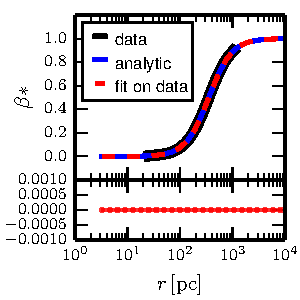
\includegraphics[width=0.4\textwidth]{fig/beta_fit_all.pdf}
        \caption{Fitting of the analytic $\beta$ profile using the form in
          equation \ref{eqn:nonparbetastar}. The upper plot shows an analytic
          Osipkov-Merrit anisotropy profile as dashed, black curve, and our
          fitted profile. Shown below is the difference between analytic and
          fitted profile. We see that the analytic profile is fit well over the
          range of input data, and extrapolated agreeably well to higher radii.}
        \label{fig:betafitting}
    \end{center}
\end{figure}

The anisotropy parameters for the fourth order moments ($\beta'$) are assumed to
be constant over all radii. A further refinement of our method will include
binwise changing $\beta'$ and the use virial parameters as introduced in
\cite{RichardsonFairbairn2014}.

\subsection{Comparison with data}\label{sec:datacompare}

Given the above functional forms, $\siglosi(r)$ is calculated from $\rho(r)$,
$\nu_i(r)$, and $\beta_i(r)$ according to equation \ref{eqn:LOS}. This is done
numerically, involving three integrations, which are performed with polynomial
extrapolations of the integrands up to infinity, such that missing contributions
from $r>r_{\text max}$ do not lead to an artificial falloff of $\siglos$.

The last step involves comparison of the projected surface density $\Sigma_i(r)$
-- calculated from the 3D tracer density $\nu_i(r)$ -- as well as $\sigma_{{\rm
    LOS},i}(r)$, to the respective 2D data profiles for the tracer
populations. We use a likelihood based on the overall goodness of fit:

\begin{eqnarray}
    \chi^2 &=& \sum_{i=1}^N \chi_{\Sigma,i}^2 + \chi_{\sigma,i}^2,\\
    \chi_{\Sigma,i}^2 &=& \sum_{j=1}^{N_{\rm bin}} \left(\frac{\Sigma_{\text{data},i}(r_j)-\Sigma_{\text{model},i}(r_j)}{\varepsilon_\Sigma(r_j)}\right)^2,
\end{eqnarray}
with error $\varepsilon_\Sigma(r_j)$ on the data
$\Sigma_{\text{data},i}(r_j)$. Analogous expressions hold for
$\chi_{\sigma,i}^2$. In the absence of a
measured $\beta_i(r)$, we set $\chi_{\beta,i}^2=0$.

\subsection{Priors}

We investigate two theoretically motivated priors on the dark matter density
profile:

\begin{enumerate}
    \item A regularization prior on $n(r)$:
    $|n(r_{j+1})-n(r_{j})|/(\ln(r_{j+1})-\ln(r_{j}))<f\cdot\frac{\ln(r_{\rm
        max})}{N_{\rm bin}}$ with a tuning factor $f$ of order
    unity. This is designed to prevent $n(r)$ fluctuating wildly from bin to bin.

    \item An absolute prior on $n(r)$: $n(r<r_{1/2})<2.0$. This corresponds to a
    prior that the stars in the galaxy lie deep within their host dark matter
    halo (since at large radii, the dark matter halo is expected to have a slope
    of $n = 3$).
\end{enumerate}
Both priors can be switched; we explore their effect in \S\ref{sec:results}.

Otherwise, we use very weak flat priors on all other parameters:

\begin{enumerate}
    \item[1)] $0\leq \rho_{{\rm DM},j} \leq 5$
    \item[2)] $0\leq \nu_{i,j}  \leq 5$
    \item[3)] $0\leq b_{i,j} \leq 10$
\end{enumerate}
where $\rho_{{\rm DM},j}$ and $\nu_{i,j}$ are the dark matter density and tracer
density (for population $i$) in bin $j$; and $b_{i,j}$ is the polynomial
coefficient $b_j$ for tracer population $i$.

%\subsection{Non-Parametric Representation}
%
%There are a large number of parameters from the representation of the profiles,
%
%\begin{equation}
%    N_{\rm dim} = N_{\rm bin} + N_{\rm pop}\cdot(N_{\rm bin}+N_{\rm beta})
%\end{equation}
%
%with only very few constraints from physical priors. The functional
%form of the profiles is not predescribed. These conditions represent
%what we call a {\it non-parametric representation}.

\subsection{Parameter Space Sampling}
Given the freedom in our function forms for the matter density; tracer
densities; and the velocity anisotropy profiles of these, we are left with a
large number of free parameters:

\begin{equation}
    N_{\rm dim} = N_{\rm bin} + N_{\rm pop}\cdot(N_{\rm bin}+N_{\rm beta})
\end{equation}
with significantly fewer observational constraints. As discussed in
\S\ref{sec:introduction}, we refer to this as `non-parametric' mass modelling.

To efficiently sample the above high dimensional parameter space, we use the
\MultiNest\ code \citep{FerozHobson2008}, \citep{Feroz+2009},
\citep{Feroz+2013}, see also
\url{http://ccpforge.cse.rl.ac.uk/gf/project/multinest/}. This is a Bayesian
nested sampling algorithm to generate posterior samples from non-trivial
distributions in high dimensions. \MultiNest\ samples the $n$-dimensional
hypercube $\kappa=[0,1]^{N_{\rm dim}}$, which needs to be translated into
physical prior distributions for each of the parameter profiles.

%%% Local Variables:
%%% mode: latex
%%% TeX-master: "Steger_2014_Gravlite"
%%% End:
